\definecolor{mycolor1}{rgb}{0.00000,0.44700,0.74100}%
\definecolor{mycolor2}{rgb}{0.85000,0.32500,0.09800}%

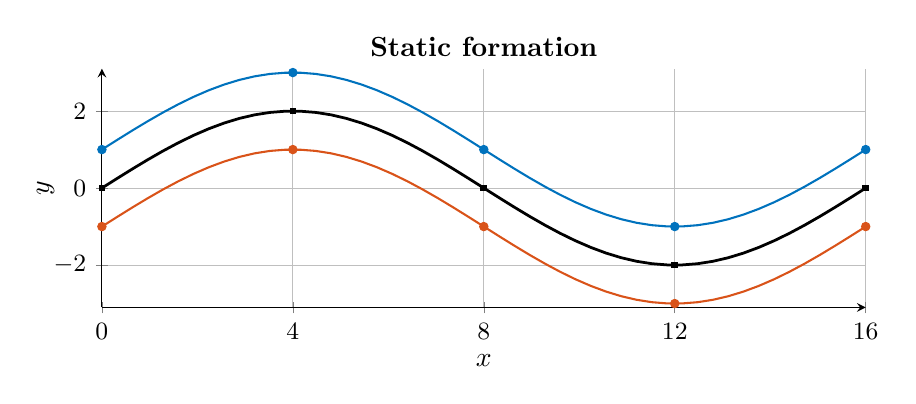
\begin{tikzpicture}
\begin{axis}[
    width=0.8\textwidth,
    height=0.25\textwidth,
    scale only axis,
    axis lines=left,
    xlabel=$x$,
    xlabel style={yshift=0.5mm},
    ylabel=$y$,
    ylabel style={yshift=-2.5mm},
    xmin=0,
    xmax=16,
    xtick={0,4,8,12,16},
    ymin=-3.1,
    ymax=3.1,
    xmajorgrids,
    ymajorgrids,
    title style={font=\bfseries, yshift=-1.75mm},
    title={Static formation},
    tick label style={font=\small},
]

\addplot[
    domain=0:16,
    samples=51,
    color=black,
    line width=1pt,
]
{2*sin((180/8)*x)};

\addplot[
    domain=0:16,
    samples=51,
    color=mycolor1,
    line width=0.75pt,
]
{2*sin((180/8)*x) + 1};

\addplot[
    domain=0:16,
    samples=51,
    color=mycolor2,
    line width=0.75pt,
]
{2*sin((180/8)*x) - 1};

\addplot[only marks, mark size=1pt, mark=square*, draw=black, fill=black]
table {
    0 0
    4 2
    8 0
    12 -2
    16 0
};

\addplot[only marks, mark size=1.5pt, mark=*, draw=mycolor1, fill=mycolor1]
table {
    0 1
    4 3
    8 1
    12 -1
    16 1
};

\addplot[only marks, mark size=1.5pt, mark=*, draw=mycolor2, fill=mycolor2]
table {
    0 -1
    4 1
    8 -1
    12 -3
    16 -1
};
    
\end{axis}
\end{tikzpicture}